\documentclass[dvipsnames]{article}
\usepackage{tikz,pgfplots}
\usepackage{tikz-qtree}
\usepackage{units}
\usepackage{braket}
\usepackage[]{xcolor}
\pgfplotsset{compat=1.14}
%\pgfplotsset{colormap={mix}{
%	color(0cm)=(blue);
%	color(1cm)=(green);
%	color(2cm)=(yellow)
%	color(3cm)=(red)}}

\usetikzlibrary{patterns,shadows,fadings,positioning,trees,calc}
\usepgfplotslibrary{groupplots}
\usepgfplotslibrary{external}
\tikzexternalize


\tikzfading[name=fade inside,
         inner color=transparent!80,
         outer color=transparent!30]
\tikzfading[name=fade out,
         inner color=transparent!0,
         outer color=transparent!90]


%\definecolor{diplom1}{rgb}{0.0 0.4 1.0}
%\definecolor{diplom2}{rgb}{0.0 0.0 0.6}
\definecolor{diplom1}{RGB}{101 156 239}
\definecolor{diplom2}{RGB}{000 000 128}
\definecolor{diplom3}{RGB}{153,0,0} %unirot
\definecolor{diplom4}{RGB}{232,215,23}
\definecolor{diplom5}{RGB}{51,37,60}

\definecolor{unirot}{RGB}{153,0,0}
\definecolor{unirot_hell}{RGB}{255,228,225}
\definecolor{lightblue}{RGB}{242.2,249.88,255}

\pgfplotsset{colormap={diplom1s}{
       color(0cm)=(white);
       color(1cm)=(diplom1);
       color(10cm)=(diplom1)}}
\pgfplotsset{colormap={diplom2s}{
       color(0cm)=(white);
       color(1cm)=(diplom1);
       color(2cm)=(diplom2)}}
\pgfplotsset{colormap={blues}{
       color(0cm)=(diplom2);
       color(1cm)=(diplom1);
       color(2cm)=(white);
       color(3cm)=(diplom1);
       color(4cm)=(diplom2)}}

\pgfplotsset{
   /pgfplots/bar cycle list/.style={/pgfplots/cycle list={%
        {diplom1,  fill=diplom1!30!white,  mark=none,very thick},%
        {diplom2,  fill=diplom2!30!white,  mark=none,very thick},%
        {diplom3,  fill=diplom3!30!white,  mark=none,very thick},%
        {orange,   fill=orange!30!white,   mark=none,very thick},%
        {LimeGreen,fill=LimeGreen!30!white,mark=none,very thick},%
        {Fuchsia,  fill=Fuchsia!30!white,  mark=none,very thick},%
        {Green,    fill=Green!30!white,    mark=none,very thick},%
        {Goldenrod,fill=Goldenrod!30!white,mark=none,very thick},%
     }
   },
}

\pgfplotscreateplotcyclelist{diplom}{
diplom1,every mark/.append style={fill=diplom1!30!white},mark=*\\
diplom2,every mark/.append style={fill=diplom2!30!white},mark=*\\
diplom3,every mark/.append style={fill=diplom3!30!white},mark=*\\
orange,every mark/.append style={fill=orange!30!white},mark=*\\
LimeGreen,every mark/.append style={fill=LimeGreen!30!white},mark=*\\
Fuchsia,every mark/.append style={fill=Fuchsia!30!white},mark=*\\
Green,every mark/.append style={fill=Green!30!white},mark=*\\
Goldenrod,every mark/.append style={fill=Goldenrod!30!white},mark=*\\
}

\begin{document}

%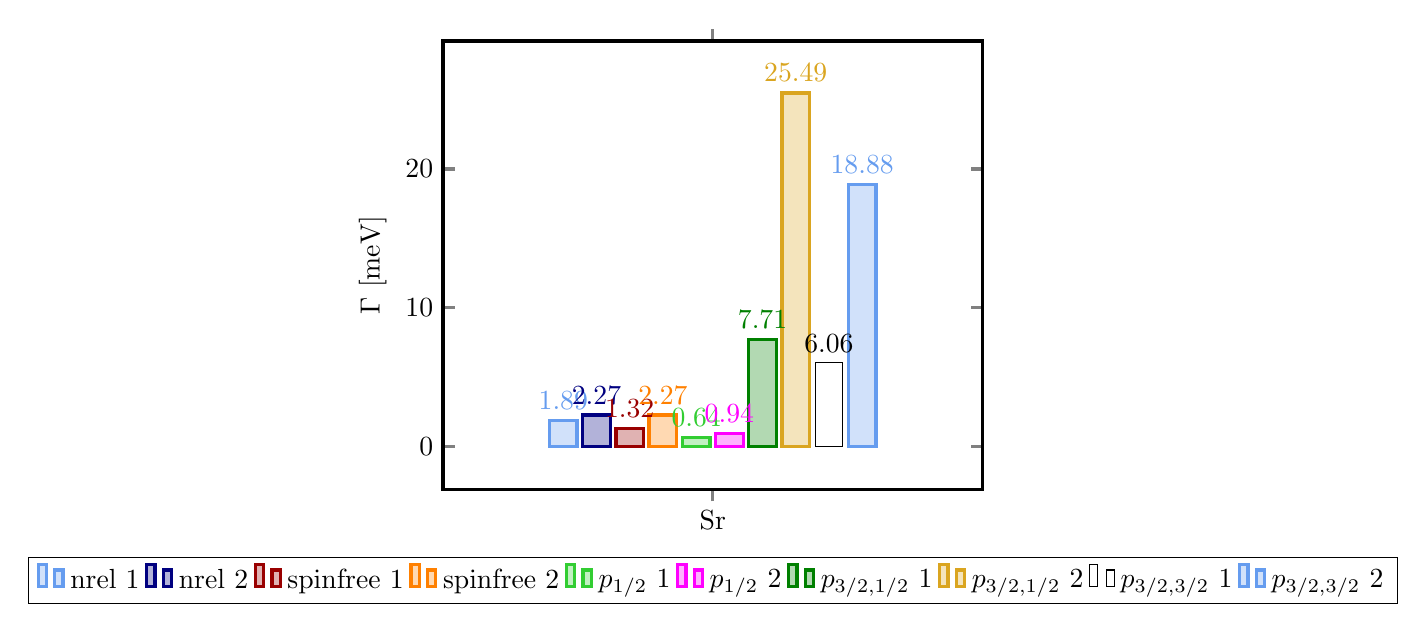
\begin{tikzpicture}
\begin{axis}[
    ybar,
    enlargelimits=0.15,
    legend style={at={(0.5,-0.15)},
      anchor=north,legend columns=-1},
    ylabel={$\Gamma$ [meV]},
    %ylabel={\#participants},
    symbolic x coords={Sr},
    xtick=data,
    nodes near coords,
    nodes near coords align={vertical},
    enlarge x limits=0.25, %space left and right
    axis line style = very thick,
    tick style = very thick
    ]
\addplot coordinates {(Sr,1.888)};
\addplot coordinates {(Sr,2.274)};
\addplot coordinates {(Sr,1.321)};
\addplot coordinates {(Sr,2.269)};
\addplot coordinates {(Sr,0.635)};
\addplot coordinates {(Sr,0.940)};
\addplot coordinates {(Sr,7.712)};
\addplot coordinates {(Sr,25.49)};
\addplot coordinates {(Sr,6.064)};
\addplot coordinates {(Sr,18.88)};
\legend{nrel 1,nrel 2,spinfree 1,spinfree 2,$p_{1/2}$ 1,$p_{1/2}$ 2,$p_{3/2,1/2}$ 1,$p_{3/2,1/2}$ 2,$p_{3/2,3/2}$ 1,$p_{3/2,3/2}$ 2};
\end{axis}
\end{tikzpicture}


%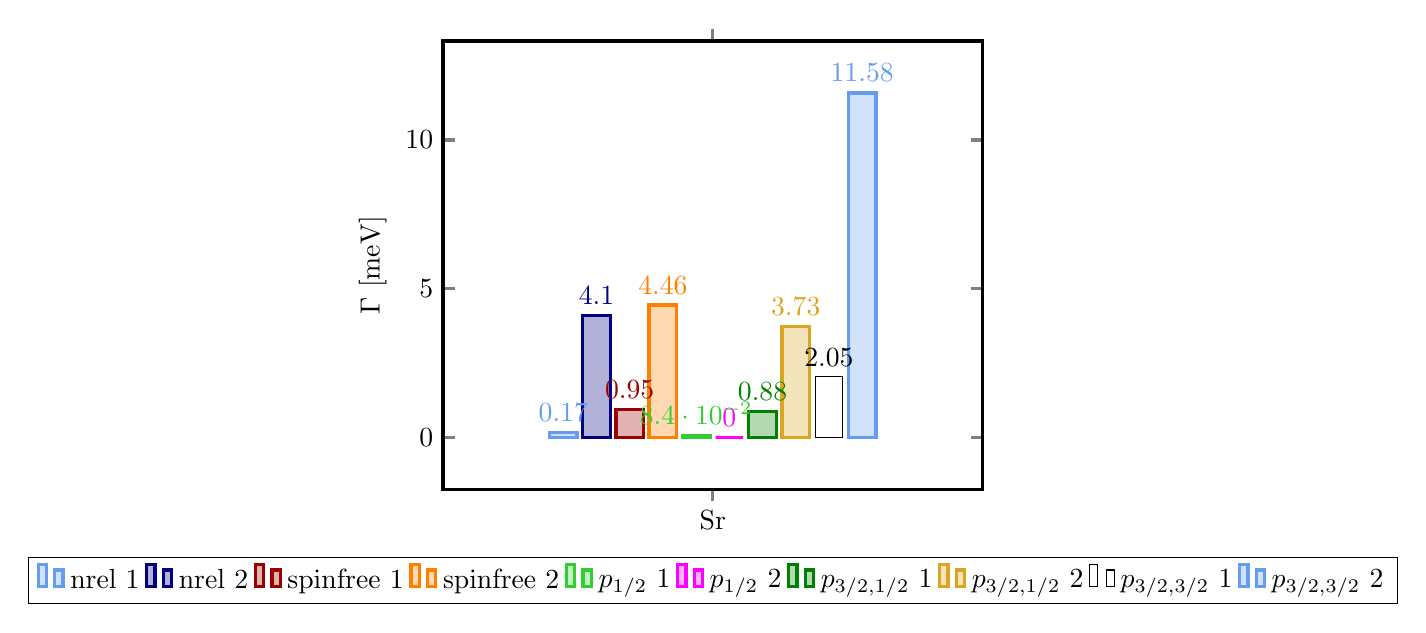
\begin{tikzpicture}
\begin{axis}[
    ybar,
    enlargelimits=0.15,
    legend style={at={(0.5,-0.15)},
      anchor=north,legend columns=-1},
    ylabel={$\Gamma$ [meV]},
    %ylabel={\#participants},
    symbolic x coords={Sr},
    xtick=data,
    nodes near coords,
    nodes near coords align={vertical},
    enlarge x limits=0.25, %space left and right
    axis line style = very thick,
    tick style = very thick
    ]
\addplot coordinates {(Sr,0.170)};
\addplot coordinates {(Sr,4.097)};
\addplot coordinates {(Sr,0.946)};
\addplot coordinates {(Sr,4.460)};
\addplot coordinates {(Sr,0.084)};
\addplot coordinates {(Sr,0.000)};
\addplot coordinates {(Sr,0.878)};
\addplot coordinates {(Sr,3.727)};
\addplot coordinates {(Sr,2.048)};
\addplot coordinates {(Sr,11.58)};
\legend{nrel 1,nrel 2,spinfree 1,spinfree 2,$p_{1/2}$ 1,$p_{1/2}$ 2,$p_{3/2,1/2}$ 1,$p_{3/2,1/2}$ 2,$p_{3/2,3/2}$ 1,$p_{3/2,3/2}$ 2};
\end{axis}
\end{tikzpicture}

\\

%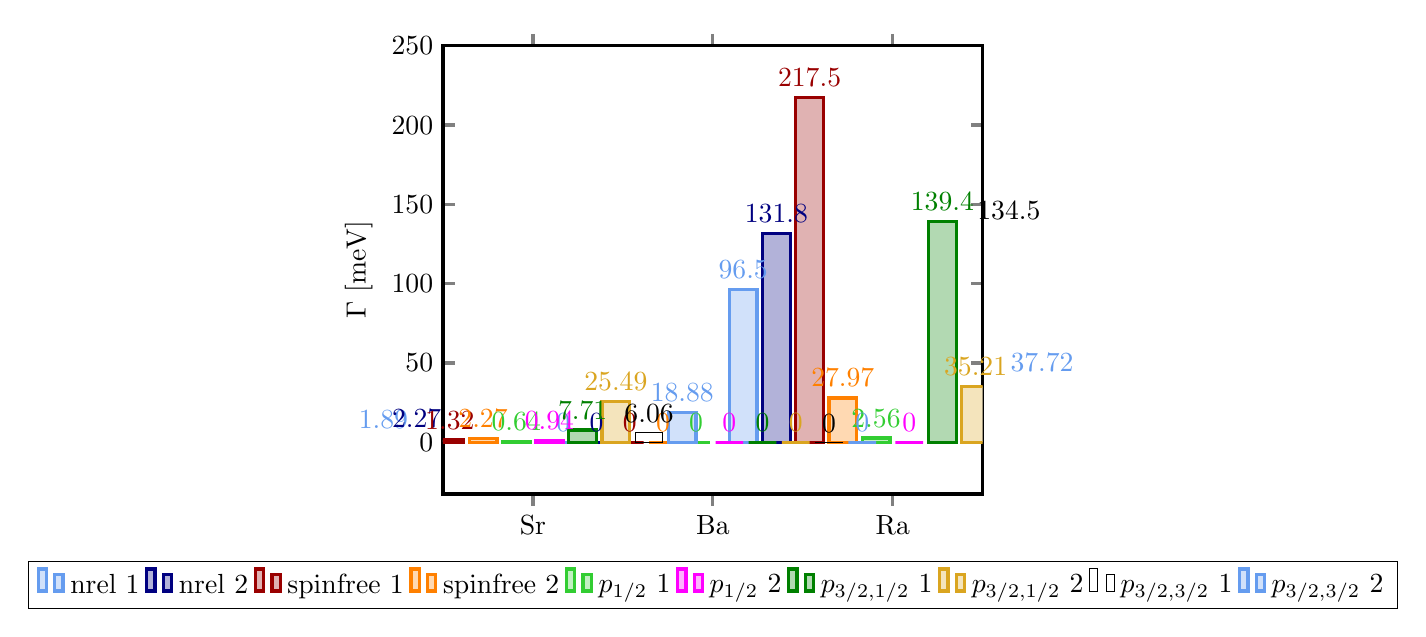
\begin{tikzpicture}
\begin{axis}[
    ybar,
    enlargelimits=0.15,
    legend style={at={(0.5,-0.15)},
      anchor=north,legend columns=-1},
    ylabel={$\Gamma$ [meV]},
    %ylabel={\#participants},
    symbolic x coords={Sr,Ba,Ra},
    xtick=data,
    nodes near coords,
    nodes near coords align={vertical},
    enlarge x limits=0.25, %space left and right
    axis line style = very thick,
    tick style = very thick
    ]
\addplot coordinates {(Sr,1.888) (Ba,0) (Ra,96.50)};
\addplot coordinates {(Sr,2.274) (Ba,0) (Ra,131.8)};
\addplot coordinates {(Sr,1.321) (Ba,0) (Ra,217.5)};
\addplot coordinates {(Sr,2.269) (Ba,0) (Ra,27.97)};
\addplot coordinates {(Sr,0.635) (Ba,0) (Ra,2.564)};
\addplot coordinates {(Sr,0.940) (Ba,0) (Ra,0)};
\addplot coordinates {(Sr,7.712) (Ba,0) (Ra,139.4)};
\addplot coordinates {(Sr,25.49) (Ba,0) (Ra,35.21)};
\addplot coordinates {(Sr,6.064) (Ba,0) (Ra,134.5)};
\addplot coordinates {(Sr,18.88) (Ba,0) (Ra,37.72)};
\legend{nrel 1,nrel 2,spinfree 1,spinfree 2,$p_{1/2}$ 1,$p_{1/2}$ 2,$p_{3/2,1/2}$ 1,$p_{3/2,1/2}$ 2,$p_{3/2,3/2}$ 1,$p_{3/2,3/2}$ 2};
\end{axis}
\end{tikzpicture}

\\
%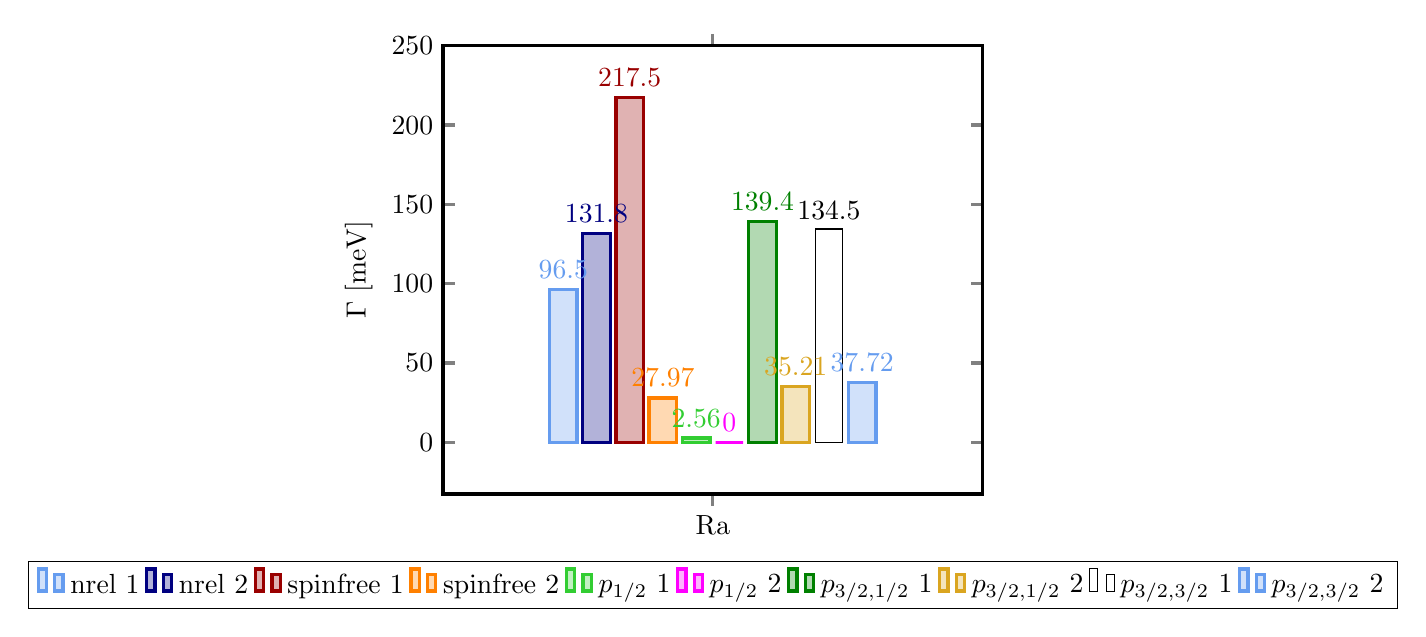
\begin{tikzpicture}
\begin{axis}[
    ybar,
    enlargelimits=0.15,
    legend style={at={(0.5,-0.15)},
      anchor=north,legend columns=-1},
    ylabel={$\Gamma$ [meV]},
    %ylabel={\#participants},
    symbolic x coords={Ra},
    xtick=data,
    nodes near coords,
    nodes near coords align={vertical},
    enlarge x limits=0.25, %space left and right
    axis line style = very thick,
    tick style = very thick
    ]
\addplot coordinates {(Ra,96.50)};
\addplot coordinates {(Ra,131.8)};
\addplot coordinates {(Ra,217.5)};
\addplot coordinates {(Ra,27.97)};
\addplot coordinates {(Ra,2.564)};
\addplot coordinates {(Ra,0)};
\addplot coordinates {(Ra,139.4)};
\addplot coordinates {(Ra,35.21)};
\addplot coordinates {(Ra,134.5)};
\addplot coordinates {(Ra,37.72)};
\legend{nrel 1,nrel 2,spinfree 1,spinfree 2,$p_{1/2}$ 1,$p_{1/2}$ 2,$p_{3/2,1/2}$ 1,$p_{3/2,1/2}$ 2,$p_{3/2,3/2}$ 1,$p_{3/2,3/2}$ 2};
\end{axis}
\end{tikzpicture}


%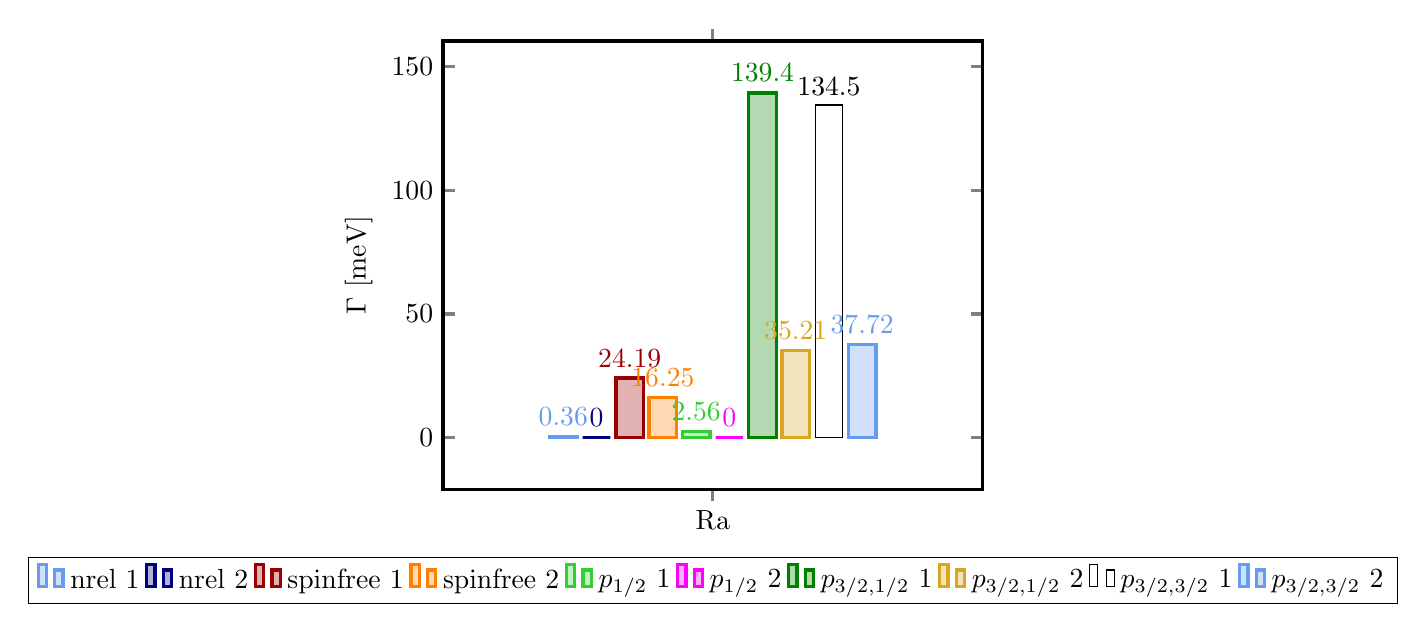
\begin{tikzpicture}
\begin{axis}[
    ybar,
    enlargelimits=0.15,
    legend style={at={(0.5,-0.15)},
      anchor=north,legend columns=-1},
    ylabel={$\Gamma$ [meV]},
    %ylabel={\#participants},
    symbolic x coords={Ra},
    xtick=data,
    nodes near coords,
    nodes near coords align={vertical},
    enlarge x limits=0.25, %space left and right
    axis line style = very thick,
    tick style = very thick
    ]
\addplot coordinates {(Ra,0.358)};
\addplot coordinates {(Ra,0.000)};
\addplot coordinates {(Ra,24.19)};
\addplot coordinates {(Ra,16.25)};
\addplot coordinates {(Ra,2.564)};
\addplot coordinates {(Ra,0)};
\addplot coordinates {(Ra,139.4)};
\addplot coordinates {(Ra,35.21)};
\addplot coordinates {(Ra,134.5)};
\addplot coordinates {(Ra,37.72)};
\legend{nrel 1,nrel 2,spinfree 1,spinfree 2,$p_{1/2}$ 1,$p_{1/2}$ 2,$p_{3/2,1/2}$ 1,$p_{3/2,1/2}$ 2,$p_{3/2,3/2}$ 1,$p_{3/2,3/2}$ 2};
\end{axis}
\end{tikzpicture}


%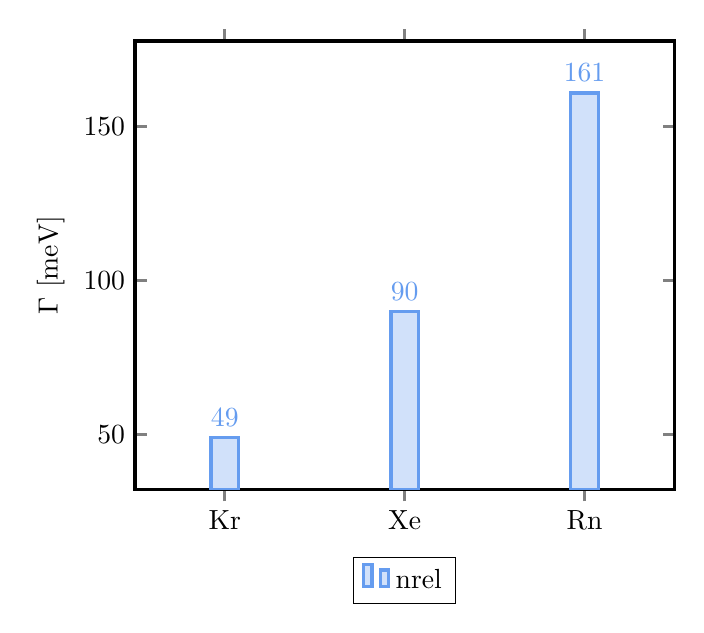
\begin{tikzpicture}
\begin{axis}[
    ybar,
    enlargelimits=0.15,
    legend style={at={(0.5,-0.15)},
      anchor=north,legend columns=-1},
    ylabel={$\Gamma$ [meV]},
    %ylabel={\#participants},
    symbolic x coords={Kr,Xe,Rn},
    xtick=data,
    nodes near coords,
    nodes near coords align={vertical},
    enlarge x limits=0.25, %space left and right
    axis line style = very thick,
    tick style = very thick
    ]
\addplot coordinates {(Kr,49) (Xe,90) (Rn,161)};
%\addplot coordinates {(Kr,62) (Xe,168) (Rn,686)};
%\addplot coordinates {(Kr,56) (Xe,132) (Rn,547)};
%\addplot coordinates {(Kr,63) (Xe,162) (Rn,624)};
\legend{nrel,spinfree,$d_{3/2}$,$d_{5/2}$}
\end{axis}
\end{tikzpicture}



%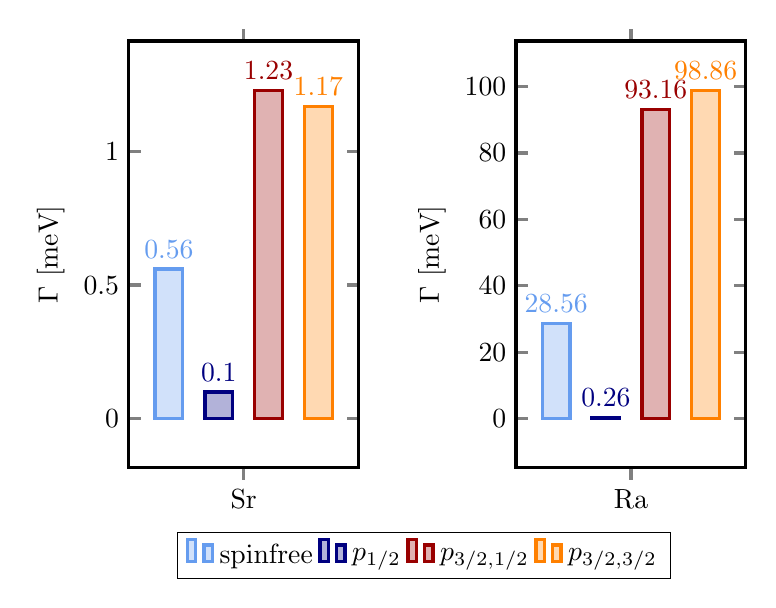
\begin{tikzpicture}
\begin{groupplot}[
     group style = {group size = 2 by 1, horizontal sep=2cm},
     enlargelimits=0.15,
     height = 7cm,
     width = 4.5cm,
     ybar = 8pt,
     legend style={at={(-0.4,-0.15)},
       anchor=north,legend columns=-1},
     ylabel={$\Gamma$ [meV]},
     symbolic x coords={Sr,Ra},
     xtick=data,
     nodes near coords,
     nodes near coords align={vertical},
     enlarge x limits=0.20, %space left and right
     axis line style = very thick,
     tick style = very thick,
    ]
    \nextgroupplot[ymin=0]
    \addplot coordinates {(Sr,0.56) };
    \addplot coordinates {(Sr,0.10) };
    \addplot coordinates {(Sr,1.23) };
    \addplot coordinates {(Sr,1.17) };

    \nextgroupplot[ymin=0]
    \addplot coordinates { (Ra,28.56)};
    \addplot coordinates { (Ra,0.26)};
    \addplot coordinates { (Ra,93.16)};
    \addplot coordinates { (Ra,98.86)};
\legend{spinfree,$p_{1/2}$,$p_{3/2,1/2}$,$p_{3/2,3/2}$};
  \end{groupplot}
\end{tikzpicture}




%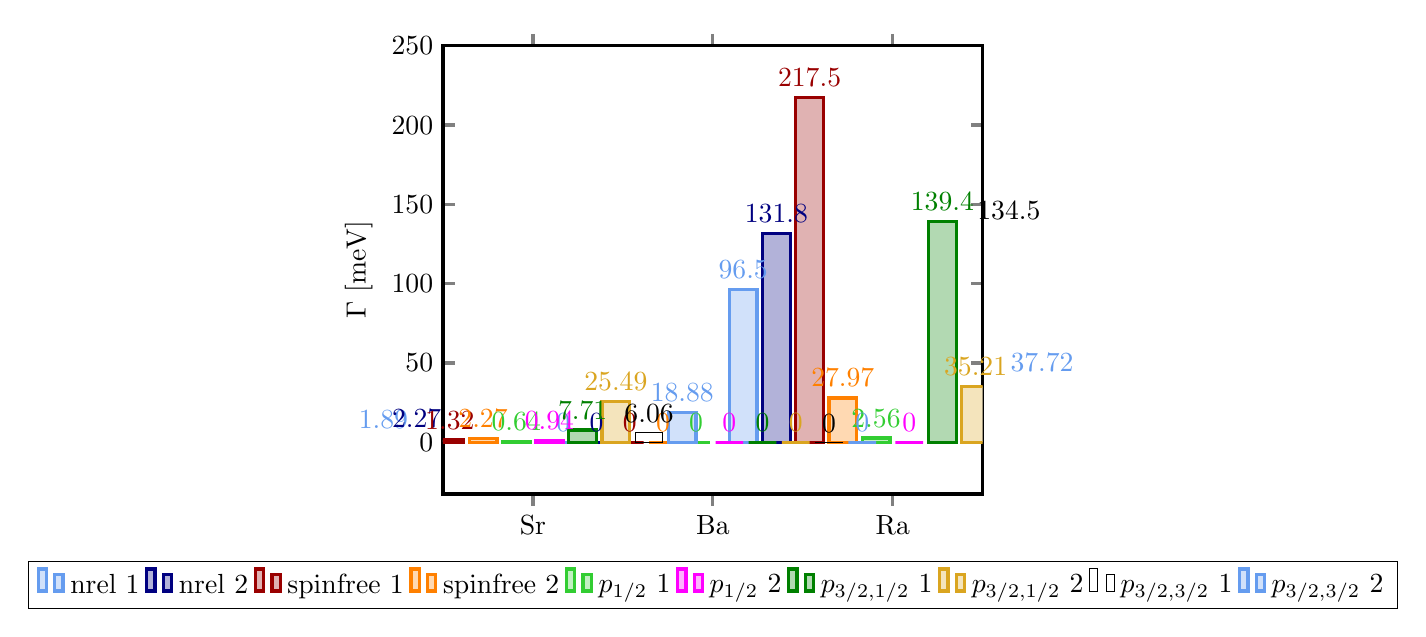
\begin{tikzpicture}
\begin{axis}[
    ybar,
    enlargelimits=0.15,
    legend style={at={(0.5,-0.15)},
      anchor=north,legend columns=-1},
    ylabel={$\Gamma$ [meV]},
    %ylabel={\#participants},
    symbolic x coords={Sr,Ba,Ra},
    xtick=data,
    nodes near coords,
    nodes near coords align={vertical},
    enlarge x limits=0.25, %space left and right
    axis line style = very thick,
    tick style = very thick
    ]
\addplot coordinates {(Sr,1.888) (Ba,0) (Ra,96.50)};
\addplot coordinates {(Sr,2.274) (Ba,0) (Ra,131.8)};
\addplot coordinates {(Sr,1.321) (Ba,0) (Ra,217.5)};
\addplot coordinates {(Sr,2.269) (Ba,0) (Ra,27.97)};
\addplot coordinates {(Sr,0.635) (Ba,0) (Ra,2.564)};
\addplot coordinates {(Sr,0.940) (Ba,0) (Ra,0)};
\addplot coordinates {(Sr,7.712) (Ba,0) (Ra,139.4)};
\addplot coordinates {(Sr,25.49) (Ba,0) (Ra,35.21)};
\addplot coordinates {(Sr,6.064) (Ba,0) (Ra,134.5)};
\addplot coordinates {(Sr,18.88) (Ba,0) (Ra,37.72)};
\legend{nrel 1,nrel 2,spinfree 1,spinfree 2,$p_{1/2}$ 1,$p_{1/2}$ 2,$p_{3/2,1/2}$ 1,$p_{3/2,1/2}$ 2,$p_{3/2,3/2}$ 1,$p_{3/2,3/2}$ 2};
\end{axis}
\end{tikzpicture}



%\begin{tikzpicture}[scale=1.0]

\begin{axis}[%scale=1.5,
             domain=0:1.4,
             restrict expr to domain={x}{0:1.4},
             %restrict expr to domain={y}{1.0E-12:7},
             xlabel={r [\AA]},
             %xtick={30,50,...,170},
             %xticklabels={2,4,6,8,10,12,15,20,25},
             %ytick={-1.0,-0.8,...,1.0},
             %yticklabels={1.0,0.8,0.6,0.4,0.2,0.0,0.2,0.4,0.6,0.8,1.0},
             ylabel={$P(r)^2 + Q(r)^2$},
             scale only axis,
             width=12cm,
             height=8cm,
             %ybar stacked
             cycle list name = diplom,
             legend cell align=right,
             axis line style = very thick,
             tick style = very thick
             ]


\addplot+[
         mark=none,
         %color=diplom1,
         very thick
         ]
         table[
         x expr= 0.529 * (\thisrowno{1}),
         y expr={(\thisrowno{6})^2 + (\thisrowno{7})^2}
         ]
         {../data/ne_radial.dat};
         \addlegendentry{Ne rel. 2$p_{1/2}$};

\addplot+[
         mark=none,
         %color=diplom1,
         very thick
         ]
         table[
         x expr= 0.529 * (\thisrowno{1}),
         y expr={(\thisrowno{8})^2 + (\thisrowno{9})^2}
         ]
         {../data/ne_radial.dat};
         \addlegendentry{Ne rel. 2$p_{3/2}$};

%\addplot+[
%         mark=none,
%         %color=diplom1,
%         very thick
%         ]
%         table[
%         x expr= 0.529 * (\thisrowno{1}),
%         y expr={(\thisrowno{2})^2 + (\thisrowno{3})^2}
%         ]
%         {../data/sr_5s.dat};
%         \addlegendentry{Ne rel. 5$s$};

%\addplot+[
%         mark=none,
%         %color=diplom2,
%         very thick
%         ]
%         table[
%         x expr= 0.529 * (\thisrowno{1}),
%         y expr={(\thisrowno{4})^2 + (\thisrowno{5})^2}
%         ]
%         {../data/P_xe_nrel_outer.dat};
%         \addlegendentry{Xe nrel. 4d};
%
%
%%s
%\addplot+[
%         mark=none,
%         %color=diplom1,
%         very thick
%         ]
%         table[
%         x expr= 0.529 * (\thisrowno{1}),
%         y expr={(\thisrowno{6})^2 + (\thisrowno{7})^2}
%         ]
%         {../data/P_xe_rel_outer.dat};
%         \addlegendentry{Xe rel. 5s};
%
%\addplot+[
%         mark=none,
%         %color=diplom2,
%         very thick
%         ]
%         table[
%         x expr= 0.529 * (\thisrowno{1}),
%         y expr={(\thisrowno{6})^2 + (\thisrowno{7})^2}
%         ]
%         {../data/P_xe_nrel_outer.dat};
%         \addlegendentry{Xe nrel. 5s};
%
%%p
%\addplot+[
%         mark=none,
%         %color=diplom1,
%         very thick
%         ]
%         table[
%         x expr= 0.529 * (\thisrowno{1}),
%         y expr={(\thisrowno{8})^2 + (\thisrowno{9})^2}
%         ]
%         {../data/P_xe_rel_outer.dat};
%         \addlegendentry{Xe rel. 5p};
%
%\addplot+[
%         mark=none,
%         %color=diplom2,
%         very thick
%         ]
%         table[
%         x expr= 0.529 * (\thisrowno{1}),
%         y expr={(\thisrowno{8})^2 + (\thisrowno{9})^2}
%         ]
%         {../data/P_xe_nrel_outer.dat};
%         \addlegendentry{Xe nrel. 5p};


\end{axis}
\end{tikzpicture}

%\begin{tikzpicture}[scale=1.0]

\begin{axis}[%scale=1.5,
             domain=0:2.5,
             restrict expr to domain={x}{0:2.5},
             %restrict expr to domain={y}{1.0E-12:7},
             xlabel={r [\AA]},
             %xtick={30,50,...,170},
             %xticklabels={2,4,6,8,10,12,15,20,25},
             %ytick={-1.0,-0.8,...,1.0},
             %yticklabels={1.0,0.8,0.6,0.4,0.2,0.0,0.2,0.4,0.6,0.8,1.0},
             ylabel={$P(r)^2 + Q(r)^2$},
             scale only axis,
             width=12cm,
             height=8cm,
             %ybar stacked
             cycle list name = diplom,
             legend cell align=right,
             axis line style = very thick,
             tick style = very thick
             ]


\addplot+[
         mark=none,
         %color=diplom1,
         very thick
         ]
         table[
         x expr= 0.529 * (\thisrowno{1}),
         y expr={(\thisrowno{6})^2 + (\thisrowno{7})^2}
         ]
         {../data/sr_4p.dat};
         \addlegendentry{Sr rel. 4$p_{1/2}$};

\addplot+[
         mark=none,
         %color=diplom1,
         very thick
         ]
         table[
         x expr= 0.529 * (\thisrowno{1}),
         y expr={(\thisrowno{8})^2 + (\thisrowno{9})^2}
         ]
         {../data/sr_4p.dat};
         \addlegendentry{Sr rel. 4$p_{3/2}$};

\addplot+[
         mark=none,
         %color=diplom1,
         very thick
         ]
         table[
         x expr= 0.529 * (\thisrowno{1}),
         y expr={(\thisrowno{2})^2 + (\thisrowno{3})^2}
         ]
         {../data/sr_5s.dat};
         \addlegendentry{Sr rel. 5$s$};

%\addplot+[
%         mark=none,
%         %color=diplom2,
%         very thick
%         ]
%         table[
%         x expr= 0.529 * (\thisrowno{1}),
%         y expr={(\thisrowno{4})^2 + (\thisrowno{5})^2}
%         ]
%         {../data/P_xe_nrel_outer.dat};
%         \addlegendentry{Xe nrel. 4d};
%
%
%%s
%\addplot+[
%         mark=none,
%         %color=diplom1,
%         very thick
%         ]
%         table[
%         x expr= 0.529 * (\thisrowno{1}),
%         y expr={(\thisrowno{6})^2 + (\thisrowno{7})^2}
%         ]
%         {../data/P_xe_rel_outer.dat};
%         \addlegendentry{Xe rel. 5s};
%
%\addplot+[
%         mark=none,
%         %color=diplom2,
%         very thick
%         ]
%         table[
%         x expr= 0.529 * (\thisrowno{1}),
%         y expr={(\thisrowno{6})^2 + (\thisrowno{7})^2}
%         ]
%         {../data/P_xe_nrel_outer.dat};
%         \addlegendentry{Xe nrel. 5s};
%
%%p
%\addplot+[
%         mark=none,
%         %color=diplom1,
%         very thick
%         ]
%         table[
%         x expr= 0.529 * (\thisrowno{1}),
%         y expr={(\thisrowno{8})^2 + (\thisrowno{9})^2}
%         ]
%         {../data/P_xe_rel_outer.dat};
%         \addlegendentry{Xe rel. 5p};
%
%\addplot+[
%         mark=none,
%         %color=diplom2,
%         very thick
%         ]
%         table[
%         x expr= 0.529 * (\thisrowno{1}),
%         y expr={(\thisrowno{8})^2 + (\thisrowno{9})^2}
%         ]
%         {../data/P_xe_nrel_outer.dat};
%         \addlegendentry{Xe nrel. 5p};


\end{axis}
\end{tikzpicture}

%\begin{tikzpicture}[scale=1.0]

\begin{axis}[%scale=1.5,
             domain=0:2.5,
             restrict expr to domain={x}{0:2.5},
             %restrict expr to domain={y}{1.0E-12:7},
             xlabel={r [\AA]},
             %xtick={30,50,...,170},
             %xticklabels={2,4,6,8,10,12,15,20,25},
             %ytick={-1.0,-0.8,...,1.0},
             %yticklabels={1.0,0.8,0.6,0.4,0.2,0.0,0.2,0.4,0.6,0.8,1.0},
             ylabel={$P(r)^2 + Q(r)^2$},
             scale only axis,
             width=12cm,
             height=8cm,
             %ybar stacked
             cycle list name = diplom,
             legend cell align=right,
             axis line style = very thick,
             tick style = very thick
             ]


\addplot+[
         mark=none,
         %color=diplom1,
         very thick
         ]
         table[
         x expr= 0.529 * (\thisrowno{1}),
         y expr={(\thisrowno{4})^2 + (\thisrowno{5})^2}
         ]
         {../data/ba_5p.dat};
         \addlegendentry{Ba rel. 5$p_{1/2}$};

\addplot+[
         mark=none,
         %color=diplom1,
         very thick
         ]
         table[
         x expr= 0.529 * (\thisrowno{1}),
         y expr={(\thisrowno{2})^2 + (\thisrowno{3})^2}
         ]
         {../data/ba_6s.dat};
         \addlegendentry{Ba rel. 5$p_{3/2}$};

\addplot+[
         mark=none,
         %color=diplom1,
         very thick
         ]
         table[
         x expr= 0.529 * (\thisrowno{1}),
         y expr={(\thisrowno{4})^2 + (\thisrowno{5})^2}
         ]
         {../data/ba_6s.dat};
         \addlegendentry{Ba rel. 6$s$};

%\addplot+[
%         mark=none,
%         %color=diplom2,
%         very thick
%         ]
%         table[
%         x expr= 0.529 * (\thisrowno{1}),
%         y expr={(\thisrowno{4})^2 + (\thisrowno{5})^2}
%         ]
%         {../data/P_xe_nrel_outer.dat};
%         \addlegendentry{Xe nrel. 4d};
%
%
%%s
%\addplot+[
%         mark=none,
%         %color=diplom1,
%         very thick
%         ]
%         table[
%         x expr= 0.529 * (\thisrowno{1}),
%         y expr={(\thisrowno{6})^2 + (\thisrowno{7})^2}
%         ]
%         {../data/P_xe_rel_outer.dat};
%         \addlegendentry{Xe rel. 5s};
%
%\addplot+[
%         mark=none,
%         %color=diplom2,
%         very thick
%         ]
%         table[
%         x expr= 0.529 * (\thisrowno{1}),
%         y expr={(\thisrowno{6})^2 + (\thisrowno{7})^2}
%         ]
%         {../data/P_xe_nrel_outer.dat};
%         \addlegendentry{Xe nrel. 5s};
%
%%p
%\addplot+[
%         mark=none,
%         %color=diplom1,
%         very thick
%         ]
%         table[
%         x expr= 0.529 * (\thisrowno{1}),
%         y expr={(\thisrowno{8})^2 + (\thisrowno{9})^2}
%         ]
%         {../data/P_xe_rel_outer.dat};
%         \addlegendentry{Xe rel. 5p};
%
%\addplot+[
%         mark=none,
%         %color=diplom2,
%         very thick
%         ]
%         table[
%         x expr= 0.529 * (\thisrowno{1}),
%         y expr={(\thisrowno{8})^2 + (\thisrowno{9})^2}
%         ]
%         {../data/P_xe_nrel_outer.dat};
%         \addlegendentry{Xe nrel. 5p};


\end{axis}
\end{tikzpicture}

%\begin{tikzpicture}[scale=1.0]

\begin{axis}[%scale=1.5,
             domain=0:2.5,
             restrict expr to domain={x}{0:2.5},
             %restrict expr to domain={y}{1.0E-12:7},
             xlabel={r [\AA]},
             %xtick={30,50,...,170},
             %xticklabels={2,4,6,8,10,12,15,20,25},
             %ytick={-1.0,-0.8,...,1.0},
             %yticklabels={1.0,0.8,0.6,0.4,0.2,0.0,0.2,0.4,0.6,0.8,1.0},
             ylabel={$P(r)^2 + Q(r)^2$},
             scale only axis,
             width=12cm,
             height=8cm,
             %ybar stacked
             cycle list name = diplom,
             %cycle list name = exotic,
             legend cell align=right,
             axis line style = very thick,
             tick style = very thick
             ]


\addplot+[
         mark=none,
         %color=diplom1,
         very thick
         ]
         table[
         x expr= 0.529 * (\thisrowno{1}),
         y expr={(\thisrowno{4})^2 + (\thisrowno{5})^2}
         ]
         {../data/ra_6p.dat};
         \addlegendentry{Ra rel. 6$p_{1/2}$};

\addplot+[
         mark=none,
         %color=diplom1,
         very thick
         ]
         table[
         x expr= 0.529 * (\thisrowno{1}),
         y expr={(\thisrowno{6})^2 + (\thisrowno{7})^2}
         ]
         {../data/ra_6p.dat};
         \addlegendentry{Ra rel. 6$p_{3/2}$};

\addplot+[
         mark=none,
         %color=diplom1,
         very thick
         ]
         table[
         x expr= 0.529 * (\thisrowno{1}),
         y expr={(\thisrowno{2})^2 + (\thisrowno{3})^2}
         ]
         {../data/ra_7s.dat};
         \addlegendentry{Ra rel. 7$s$};

%\addplot+[
%         mark=none,
%         %color=diplom2,
%         very thick
%         ]
%         table[
%         x expr= 0.529 * (\thisrowno{1}),
%         y expr={(\thisrowno{4})^2 + (\thisrowno{5})^2}
%         ]
%         {../data/P_xe_nrel_outer.dat};
%         \addlegendentry{Xe nrel. 4d};
%
%
%%s
%\addplot+[
%         mark=none,
%         %color=diplom1,
%         very thick
%         ]
%         table[
%         x expr= 0.529 * (\thisrowno{1}),
%         y expr={(\thisrowno{6})^2 + (\thisrowno{7})^2}
%         ]
%         {../data/P_xe_rel_outer.dat};
%         \addlegendentry{Xe rel. 5s};
%
%\addplot+[
%         mark=none,
%         %color=diplom2,
%         very thick
%         ]
%         table[
%         x expr= 0.529 * (\thisrowno{1}),
%         y expr={(\thisrowno{6})^2 + (\thisrowno{7})^2}
%         ]
%         {../data/P_xe_nrel_outer.dat};
%         \addlegendentry{Xe nrel. 5s};
%
%%p
%\addplot+[
%         mark=none,
%         %color=diplom1,
%         very thick
%         ]
%         table[
%         x expr= 0.529 * (\thisrowno{1}),
%         y expr={(\thisrowno{8})^2 + (\thisrowno{9})^2}
%         ]
%         {../data/P_xe_rel_outer.dat};
%         \addlegendentry{Xe rel. 5p};
%
%\addplot+[
%         mark=none,
%         %color=diplom2,
%         very thick
%         ]
%         table[
%         x expr= 0.529 * (\thisrowno{1}),
%         y expr={(\thisrowno{8})^2 + (\thisrowno{9})^2}
%         ]
%         {../data/P_xe_nrel_outer.dat};
%         \addlegendentry{Xe nrel. 5p};


\end{axis}
\end{tikzpicture}


%\begin{tikzpicture}[scale=1.0]

\begin{axis}[%scale=1.5,
             domain=0:2.5,
             restrict expr to domain={x}{0:2.5},
             %restrict expr to domain={y}{1.0E-12:7},
             xlabel={r [\AA]},
             %xtick={30,50,...,170},
             %xticklabels={2,4,6,8,10,12,15,20,25},
             %ytick={-1.0,-0.8,...,1.0},
             %yticklabels={1.0,0.8,0.6,0.4,0.2,0.0,0.2,0.4,0.6,0.8,1.0},
             ylabel={$P(r)^2 + Q(r)^2$},
             scale only axis,
             width=12cm,
             height=8cm,
             %ybar stacked
             cycle list name = diplom,
             legend cell align=right,
             axis line style = very thick,
             tick style = very thick
             ]


\addplot+[
         mark=none,
         %color=diplom1,
         very thick
         ]
         table[
         x expr= 0.529 * (\thisrowno{1}),
         y expr={(\thisrowno{2})^2 + (\thisrowno{3})^2}
         ]
         {../data/sr_ion_4p_orb.dat};
         \addlegendentry{Sr rel. 4$p_{1/2}$};

\addplot+[
         mark=none,
         %color=diplom1,
         very thick
         ]
         table[
         x expr= 0.529 * (\thisrowno{1}),
         y expr={(\thisrowno{4})^2 + (\thisrowno{5})^2}
         ]
         {../data/sr_ion_4p_orb.dat};
         \addlegendentry{Sr rel. 4$p_{3/2}$};

\addplot+[
         mark=none,
         %color=diplom1,
         very thick
         ]
         table[
         x expr= 0.529 * (\thisrowno{1}),
         y expr={(\thisrowno{2})^2 + (\thisrowno{3})^2}
         ]
         {../data/sr_ion_5s_orb.dat};
         \addlegendentry{Sr rel. 5$s$};

%\addplot+[
%         mark=none,
%         %color=diplom2,
%         very thick
%         ]
%         table[
%         x expr= 0.529 * (\thisrowno{1}),
%         y expr={(\thisrowno{4})^2 + (\thisrowno{5})^2}
%         ]
%         {../data/P_xe_nrel_outer.dat};
%         \addlegendentry{Xe nrel. 4d};
%
%
%%s
%\addplot+[
%         mark=none,
%         %color=diplom1,
%         very thick
%         ]
%         table[
%         x expr= 0.529 * (\thisrowno{1}),
%         y expr={(\thisrowno{6})^2 + (\thisrowno{7})^2}
%         ]
%         {../data/P_xe_rel_outer.dat};
%         \addlegendentry{Xe rel. 5s};
%
%\addplot+[
%         mark=none,
%         %color=diplom2,
%         very thick
%         ]
%         table[
%         x expr= 0.529 * (\thisrowno{1}),
%         y expr={(\thisrowno{6})^2 + (\thisrowno{7})^2}
%         ]
%         {../data/P_xe_nrel_outer.dat};
%         \addlegendentry{Xe nrel. 5s};
%
%%p
%\addplot+[
%         mark=none,
%         %color=diplom1,
%         very thick
%         ]
%         table[
%         x expr= 0.529 * (\thisrowno{1}),
%         y expr={(\thisrowno{8})^2 + (\thisrowno{9})^2}
%         ]
%         {../data/P_xe_rel_outer.dat};
%         \addlegendentry{Xe rel. 5p};
%
%\addplot+[
%         mark=none,
%         %color=diplom2,
%         very thick
%         ]
%         table[
%         x expr= 0.529 * (\thisrowno{1}),
%         y expr={(\thisrowno{8})^2 + (\thisrowno{9})^2}
%         ]
%         {../data/P_xe_nrel_outer.dat};
%         \addlegendentry{Xe nrel. 5p};


\end{axis}
\end{tikzpicture}
\\
%\begin{tikzpicture}[scale=1.0]

\begin{axis}[%scale=1.5,
             domain=0:2.5,
             restrict expr to domain={x}{0:2.5},
             %restrict expr to domain={y}{1.0E-12:7},
             xlabel={r [\AA]},
             %xtick={30,50,...,170},
             %xticklabels={2,4,6,8,10,12,15,20,25},
             %ytick={-1.0,-0.8,...,1.0},
             %yticklabels={1.0,0.8,0.6,0.4,0.2,0.0,0.2,0.4,0.6,0.8,1.0},
             ylabel={$P(r)^2 + Q(r)^2$},
             scale only axis,
             width=12cm,
             height=8cm,
             %ybar stacked
             cycle list name = diplom,
             legend cell align=right,
             axis line style = very thick,
             tick style = very thick
             ]


\addplot+[
         mark=none,
         %color=diplom1,
         very thick
         ]
         table[
         x expr= 0.529 * (\thisrowno{1}),
         y expr={(\thisrowno{2})^2 + (\thisrowno{3})^2}
         ]
         {../data/ba_ion_orbs.dat};
         \addlegendentry{Ba rel. 5$p_{1/2}$};

\addplot+[
         mark=none,
         %color=diplom1,
         very thick
         ]
         table[
         x expr= 0.529 * (\thisrowno{1}),
         y expr={(\thisrowno{4})^2 + (\thisrowno{5})^2}
         ]
         {../data/ba_ion_orbs.dat};
         \addlegendentry{Ba rel. 5$p_{3/2}$};

\addplot+[
         mark=none,
         %color=diplom1,
         very thick
         ]
         table[
         x expr= 0.529 * (\thisrowno{1}),
         y expr={(\thisrowno{6})^2 + (\thisrowno{7})^2}
         ]
         {../data/ba_ion_orbs.dat};
         \addlegendentry{Ba rel. 6$s$};



\end{axis}
\end{tikzpicture}
\\
%\begin{tikzpicture}[scale=1.0]

\begin{axis}[%scale=1.5,
             domain=0:2.5,
             restrict expr to domain={x}{0:2.5},
             %restrict expr to domain={y}{1.0E-12:7},
             xlabel={r [\AA]},
             %xtick={30,50,...,170},
             %xticklabels={2,4,6,8,10,12,15,20,25},
             %ytick={-1.0,-0.8,...,1.0},
             %yticklabels={1.0,0.8,0.6,0.4,0.2,0.0,0.2,0.4,0.6,0.8,1.0},
             ylabel={$P(r)^2 + Q(r)^2$},
             scale only axis,
             width=12cm,
             height=8cm,
             %ybar stacked
             cycle list name = diplom,
             %cycle list name = exotic,
             legend cell align=right,
             axis line style = very thick,
             tick style = very thick
             ]


\addplot+[
         mark=none,
         %color=diplom1,
         very thick
         ]
         table[
         x expr= 0.529 * (\thisrowno{1}),
         y expr={(\thisrowno{2})^2 + (\thisrowno{3})^2}
         ]
         {../data/ra_ion_orbs.dat};
         \addlegendentry{Ra rel. 6$p_{1/2}$};

\addplot+[
         mark=none,
         %color=diplom1,
         very thick
         ]
         table[
         x expr= 0.529 * (\thisrowno{1}),
         y expr={(\thisrowno{4})^2 + (\thisrowno{5})^2}
         ]
         {../data/ra_ion_orbs.dat};
         \addlegendentry{Ra rel. 6$p_{3/2}$};

\addplot+[
         mark=none,
         %color=diplom1,
         very thick
         ]
         table[
         x expr= 0.529 * (\thisrowno{1}),
         y expr={(\thisrowno{6})^2 + (\thisrowno{7})^2}
         ]
         {../data/ra_ion_orbs.dat};
         \addlegendentry{Ra rel. 7$s$};

%\addplot+[
%         mark=none,
%         %color=diplom2,
%         very thick
%         ]
%         table[
%         x expr= 0.529 * (\thisrowno{1}),
%         y expr={(\thisrowno{4})^2 + (\thisrowno{5})^2}
%         ]
%         {../data/P_xe_nrel_outer.dat};
%         \addlegendentry{Xe nrel. 4d};
%
%
%%s
%\addplot+[
%         mark=none,
%         %color=diplom1,
%         very thick
%         ]
%         table[
%         x expr= 0.529 * (\thisrowno{1}),
%         y expr={(\thisrowno{6})^2 + (\thisrowno{7})^2}
%         ]
%         {../data/P_xe_rel_outer.dat};
%         \addlegendentry{Xe rel. 5s};
%
%\addplot+[
%         mark=none,
%         %color=diplom2,
%         very thick
%         ]
%         table[
%         x expr= 0.529 * (\thisrowno{1}),
%         y expr={(\thisrowno{6})^2 + (\thisrowno{7})^2}
%         ]
%         {../data/P_xe_nrel_outer.dat};
%         \addlegendentry{Xe nrel. 5s};
%
%%p
%\addplot+[
%         mark=none,
%         %color=diplom1,
%         very thick
%         ]
%         table[
%         x expr= 0.529 * (\thisrowno{1}),
%         y expr={(\thisrowno{8})^2 + (\thisrowno{9})^2}
%         ]
%         {../data/P_xe_rel_outer.dat};
%         \addlegendentry{Xe rel. 5p};
%
%\addplot+[
%         mark=none,
%         %color=diplom2,
%         very thick
%         ]
%         table[
%         x expr= 0.529 * (\thisrowno{1}),
%         y expr={(\thisrowno{8})^2 + (\thisrowno{9})^2}
%         ]
%         {../data/P_xe_nrel_outer.dat};
%         \addlegendentry{Xe nrel. 5p};


\end{axis}
\end{tikzpicture}


%\begin{tikzpicture}[scale=1.0]

\begin{axis}[%scale=1.5,
             domain=0:2.5,
             restrict expr to domain={x}{0:2.5},
             %restrict expr to domain={y}{1.0E-12:7},
             xlabel={r [\AA]},
             %xtick={30,50,...,170},
             %xticklabels={2,4,6,8,10,12,15,20,25},
             %ytick={-1.0,-0.8,...,1.0},
             %yticklabels={1.0,0.8,0.6,0.4,0.2,0.0,0.2,0.4,0.6,0.8,1.0},
             ylabel={$P(r)^2 + Q(r)^2$},
             scale only axis,
             width=12cm,
             height=8cm,
             %ybar stacked
             cycle list name = diplom,
             %cycle list name = exotic,
             legend cell align=right,
             axis line style = very thick,
             tick style = very thick
             ]


\addplot+[
         mark=none,
         %color=diplom1,
         very thick
         ]
         table[
         x expr= 0.529 * (\thisrowno{1}),
         y expr={(\thisrowno{2})^2 + (\thisrowno{3})^2}
         ]
         {../data/ra_configs/6d/ra_6.dat};
         \addlegendentry{Ra rel. 6$p_{1/2}$};

\addplot+[
         mark=none,
         %color=diplom1,
         very thick
         ]
         table[
         x expr= 0.529 * (\thisrowno{1}),
         y expr={(\thisrowno{4})^2 + (\thisrowno{5})^2}
         ]
         {../data/ra_configs/6d/ra_6.dat};
         \addlegendentry{Ra rel. 6$p_{3/2}$};

\addplot+[
         mark=none,
         %color=diplom1,
         very thick
         ]
         table[
         x expr= 0.529 * (\thisrowno{1}),
         y expr={(\thisrowno{6})^2 + (\thisrowno{7})^2}
         ]
         {../data/ra_configs/6d/ra_7.dat};
         \addlegendentry{Ra rel. 7$s$};


\addplot+[
         mark=none,
         %color=diplom1,
         very thick
         ]
         table[
         x expr= 0.529 * (\thisrowno{1}),
         y expr={(\thisrowno{2})^2 + (\thisrowno{3})^2}
         ]
         {../data/ra_configs/6d/ra_7.dat};
         \addlegendentry{Ra rel. 6$d_{3/2}$};

\addplot+[
         mark=none,
         %color=diplom1,
         very thick
         ]
         table[
         x expr= 0.529 * (\thisrowno{1}),
         y expr={(\thisrowno{4})^2 + (\thisrowno{5})^2}
         ]
         {../data/ra_configs/6d/ra_7.dat};
         \addlegendentry{Ra rel. 6$d_{5/2}$};


\end{axis}
\end{tikzpicture}

%\begin{tikzpicture}[scale=1.0]

\begin{axis}[%scale=1.5,
             domain=0:2.5,
             restrict expr to domain={x}{0:2.5},
             %restrict expr to domain={y}{1.0E-12:7},
             xlabel={r [\AA]},
             %xtick={30,50,...,170},
             %xticklabels={2,4,6,8,10,12,15,20,25},
             %ytick={-1.0,-0.8,...,1.0},
             %yticklabels={1.0,0.8,0.6,0.4,0.2,0.0,0.2,0.4,0.6,0.8,1.0},
             ylabel={$P(r)^2 + Q(r)^2$},
             scale only axis,
             width=12cm,
             height=8cm,
             %ybar stacked
             cycle list name = diplom,
             %cycle list name = exotic,
             legend cell align=right,
             axis line style = very thick,
             tick style = very thick
             ]


\addplot+[
         mark=none,
         %color=diplom1,
         very thick
         ]
         table[
         x expr= 0.529 * (\thisrowno{1}),
         y expr={(\thisrowno{2})^2 + (\thisrowno{3})^2}
         ]
         {../data/ra_configs/6d2/ra_6.dat};
         \addlegendentry{Ra rel. 6$p_{1/2}$};

\addplot+[
         mark=none,
         %color=diplom1,
         very thick
         ]
         table[
         x expr= 0.529 * (\thisrowno{1}),
         y expr={(\thisrowno{4})^2 + (\thisrowno{5})^2}
         ]
         {../data/ra_configs/6d2/ra_6.dat};
         \addlegendentry{Ra rel. 6$p_{3/2}$};


\addplot+[
         mark=none,
         %color=diplom1,
         very thick
         ]
         table[
         x expr= 0.529 * (\thisrowno{1}),
         y expr={(\thisrowno{2})^2 + (\thisrowno{3})^2}
         ]
         {../data/ra_configs/6d2/ra_7.dat};
         \addlegendentry{Ra rel. 6$d_{3/2}$};

\addplot+[
         mark=none,
         %color=diplom1,
         very thick
         ]
         table[
         x expr= 0.529 * (\thisrowno{1}),
         y expr={(\thisrowno{4})^2 + (\thisrowno{5})^2}
         ]
         {../data/ra_configs/6d2/ra_7.dat};
         \addlegendentry{Ra rel. 6$d_{5/2}$};


\end{axis}
\end{tikzpicture}


%\begin{tikzpicture}[scale=1.0]

\begin{axis}[%scale=1.5,
             domain=0:170,
             %y domain=1E-8:10,
             restrict expr to domain={x}{0:170},
             xlabel={E in \unit{eV}},
             %xtick={30,50,...,170},
             %xticklabels={2,4,6,8,10,12,15,20,25},
             ytick={-1.0,-0.8,...,1.0},
             yticklabels={1.0,0.8,0.6,0.4,0.2,0.0,0.2,0.4,0.6,0.8,1.0},
             ylabel={pole strength},
             scale only axis,
             width=\textwidth-2cm,
             height=7cm
             %title={Parameter Fitting of NeNe and NeAr Decay Widths}
             ]

\draw[gray]
  (axis cs:\pgfkeysvalueof{/pgfplots/xmin},0) --
  (axis cs:\pgfkeysvalueof{/pgfplots/xmax},0);
\addplot+[ycomb,
         %no markers,
         mark=.,
         thick,
         diplom1,
         forget plot
        ]
        table[
        x expr = \thisrowno{0},
        y expr = \thisrowno{1}
        ]
        {../data/Sr_rel_sips.dat};
        \addlegendimage{line legend, diplom1, thick};
        \addlegendentry{SIPs(Sr)};
\addplot+[ycomb,
         %no markers,
         mark=.,
         thick,
         diplom2,
         forget plot
        ]
        table[
        x expr = \thisrowno{0},
        y expr = -\thisrowno{1}
        ]
        {../data/Sr_rel_dips.dat};
        \addlegendimage{line legend, diplom2, thick};
        \addlegendentry{DIPs(Sr)};

%\node[pin={[pin distance=0.2cm]170:{\tiny 4d$_{5/2}^{-1}$}}]
%     at (axis cs:67.03,0.6) {};
%\node[pin={[pin distance=0.2cm]10:{\tiny 4d$_{3/2}^{-1}$}}]
%     at (axis cs:69.06,0.6) {};
%\node[pin={[pin distance=0.2cm]170:{\tiny 4p$_{3/2}^{-1}$}}]
%     at (axis cs:146.6,0.2) {};
%\draw[] (axis cs:165,0.15) arc [radius=0.75cm,start angle=10,end angle=100];
%\node[pin={[pin distance=0.2cm]20:{\tiny 4p$_{1/2}^{-1}$}}]
%     at (axis cs:159.6,0.23) {};
% 		
%%DIPs
%\draw[] (axis cs:39,-0.9) arc [radius=0.3cm,start angle=358,end angle=180];
%\node[pin={[pin distance=0.10cm]95:{\tiny 5p$^{-2}$}}]
%     at (axis cs:32,-0.75) {};
%
%\draw[] (axis cs:50,-0.75) arc [radius=0.3cm,start angle=358,end angle=180];
%\node[pin={[pin distance=0.05cm]280:{\tiny 5s$^{-1}$5p$^{-1}$}}]
%     at (axis cs:47,-0.80) {};
%
%\node[pin={[pin distance=0.1cm]350:{\tiny 5s$^{-2}$}}]
%     at (axis cs:59,-0.35) {};
%
%\draw[] (axis cs:96,-0.80) arc [radius=0.3cm,start angle=358,end angle=180];
%\node[pin={[pin distance=0.05cm]270:{\tiny 4d$^{-1}$5p$^{-1}$}}]
%     at (axis cs:91,-0.85) {};
%
%\draw[] (axis cs:110,-0.70) arc [radius=0.3cm,start angle=358,end angle=180];
%\node[pin={[pin distance=0.05cm]300:{\tiny 4d$^{-1}$5s$^{-1}$}}]
%     at (axis cs:106,-0.75) {};
%
%\draw[] (axis cs:165,-0.75) arc [radius=0.65cm,start angle=340,end angle=180];
%\node[pin={[pin distance=0.05cm]260:{\tiny 4d$^{-2}$}}]
%     at (axis cs:154,-0.80) {};

\end{axis}
\end{tikzpicture}

%\begin{tikzpicture}[scale=1.0]

\begin{axis}[%scale=1.5,
             %domain=0:100,
             %y domain=1E-8:10,
             %restrict expr to domain={x}{0:100},
             xmin = 0,
             xmax = 100,
             xlabel={E in \unit{eV}},
             %xtick={30,50,...,170},
             %xticklabels={2,4,6,8,10,12,15,20,25},
             ytick={-1.0,-0.8,...,1.0},
             yticklabels={1.0,0.8,0.6,0.4,0.2,0.0,0.2,0.4,0.6,0.8,1.0},
             ylabel={pole strength},
             scale only axis,
             width=\textwidth-2cm,
             height=7cm
             %title={Parameter Fitting of NeNe and NeAr Decay Widths}
             ]

\draw[gray]
  (axis cs:\pgfkeysvalueof{/pgfplots/xmin},0) --
  (axis cs:\pgfkeysvalueof{/pgfplots/xmax},0);
\addplot+[ycomb,
         %no markers,
         mark=.,
         thick,
         diplom1,
         forget plot
        ]
        table[
        x expr = \thisrowno{0},
        y expr = \thisrowno{1}
        ]
        {../data/Ra_rel_sips.dat};
        \addlegendimage{line legend, diplom1, thick};
        \addlegendentry{SIPs(Ra)};

\addplot+[ycomb,
         %no markers,
         mark=.,
         thick,
         diplom2,
         forget plot
        ]
        table[
        x expr = \thisrowno{0},
        y expr = -\thisrowno{1}
        ]
        {../data/Ra_rel_dips.dat};
        \addlegendimage{line legend, diplom2, thick};
        \addlegendentry{DIPs(Ra)};

\node[pin={[pin distance=0.2cm]10:{\tiny 7s$_{1/2}^{-1}$}}]
     at (axis cs:4.5,0.8) {};
\node[pin={[pin distance=0.2cm]170:{\tiny 6p$_{3/2}^{-1}$}}]
     at (axis cs:19.5,0.4) {};
\node[pin={[pin distance=0.2cm]10:{\tiny 6p$_{1/2}^{-1}$}}]
     at (axis cs:25.00,0.4) {};
\node[pin={[pin distance=0.2cm]10:{\tiny 6s$_{1/2}^{-1}$}}]
     at (axis cs:40.0,0.4) {};
\node[pin={[pin distance=0.2cm]190:{\tiny 7s$_{1/2}^{-2}$}}]
     at (axis cs:15.5,-0.7) {};
%\draw[] (axis cs:165,0.15) arc [radius=0.75cm,start angle=10,end angle=100];
%\node[pin={[pin distance=0.2cm]20:{\tiny 4p$_{1/2}^{-1}$}}]
%     at (axis cs:159.6,0.23) {};
% 		
%%DIPs
%\draw[] (axis cs:39,-0.9) arc [radius=0.3cm,start angle=358,end angle=180];
%\node[pin={[pin distance=0.10cm]95:{\tiny 5p$^{-2}$}}]
%     at (axis cs:32,-0.75) {};
%
%\draw[] (axis cs:50,-0.75) arc [radius=0.3cm,start angle=358,end angle=180];
%\node[pin={[pin distance=0.05cm]280:{\tiny 5s$^{-1}$5p$^{-1}$}}]
%     at (axis cs:47,-0.80) {};
%
%\node[pin={[pin distance=0.1cm]350:{\tiny 5s$^{-2}$}}]
%     at (axis cs:59,-0.35) {};
%
%\draw[] (axis cs:96,-0.80) arc [radius=0.3cm,start angle=358,end angle=180];
%\node[pin={[pin distance=0.05cm]270:{\tiny 4d$^{-1}$5p$^{-1}$}}]
%     at (axis cs:91,-0.85) {};
%
%\draw[] (axis cs:110,-0.70) arc [radius=0.3cm,start angle=358,end angle=180];
%\node[pin={[pin distance=0.05cm]300:{\tiny 4d$^{-1}$5s$^{-1}$}}]
%     at (axis cs:106,-0.75) {};
%
%\draw[] (axis cs:165,-0.75) arc [radius=0.65cm,start angle=340,end angle=180];
%\node[pin={[pin distance=0.05cm]260:{\tiny 4d$^{-2}$}}]
%     at (axis cs:154,-0.80) {};

\end{axis}
\end{tikzpicture}


%\begin{tikzpicture}[scale=1.0]

\begin{axis}[%scale=1.5,
             domain=1:120,
             %restrict expr to domain={x}{0:2.5},
             %restrict expr to domain={y}{1.0E-12:7},
             xlabel={$Z$},
             %xtick={30,50,...,170},
             %xticklabels={2,4,6,8,10,12,15,20,25},
             %ytick={-1.0,-0.8,...,1.0},
             %yticklabels={1.0,0.8,0.6,0.4,0.2,0.0,0.2,0.4,0.6,0.8,1.0},
             ylabel={$\braket{r}_{l+1/2} - \braket{r}_{l-1/2}$ [\AA]},
             scale only axis,
             width=12cm,
             height=8cm,
             xmin = 1,
             xmax = 118,
             ymin = 0,
             %ybar stacked
             cycle list name = diplom,
             %cycle list name = exotic,
             legend cell align=right,
             axis line style = very thick,
             tick style = very thick
             ]


\addplot+[
         mark=none,
         %color=diplom1,
         very thick
         ]
         table[
         x expr= (\thisrowno{0}),
         y expr={0.529 * (\thisrowno{2} - \thisrowno{1}) / 2 / \thisrowno{0}}
         ]
         {../data/comp2p.dat};
         \addlegendentry{2$p$};

\addplot+[
         mark=none,
         %color=diplom1,
         very thick
         ]
         table[
         x expr= (\thisrowno{0}),
         y expr={0.529 * (\thisrowno{2} - \thisrowno{1}) / 2 / \thisrowno{0}}
         ]
         {../data/comp3p.dat};
         \addlegendentry{3$p$};

\addplot+[
         mark=none,
         %color=diplom1,
         very thick
         ]
         table[
         x expr= (\thisrowno{0}),
         y expr={0.529 * (\thisrowno{2} - \thisrowno{1}) / 2 / \thisrowno{0}}
         ]
         {../data/comp4p.dat};
         \addlegendentry{4$p$};

\addplot+[
         mark=none,
         %color=diplom1,
         very thick
         ]
         table[
         x expr= (\thisrowno{0}),
         y expr={0.529 * (\thisrowno{2} - \thisrowno{1}) / 2 / \thisrowno{0}}
         ]
         {../data/comp6p.dat};
         \addlegendentry{6$p$};

\addplot+[
         mark=none,
         %color=diplom1,
         very thick
         ]
         table[
         x expr= (\thisrowno{0}),
         y expr={0.529 * (\thisrowno{2} - \thisrowno{1}) / 2 / \thisrowno{0}}
         ]
         {../data/comp3d.dat};
         \addlegendentry{3$d$};



\end{axis}
\end{tikzpicture}

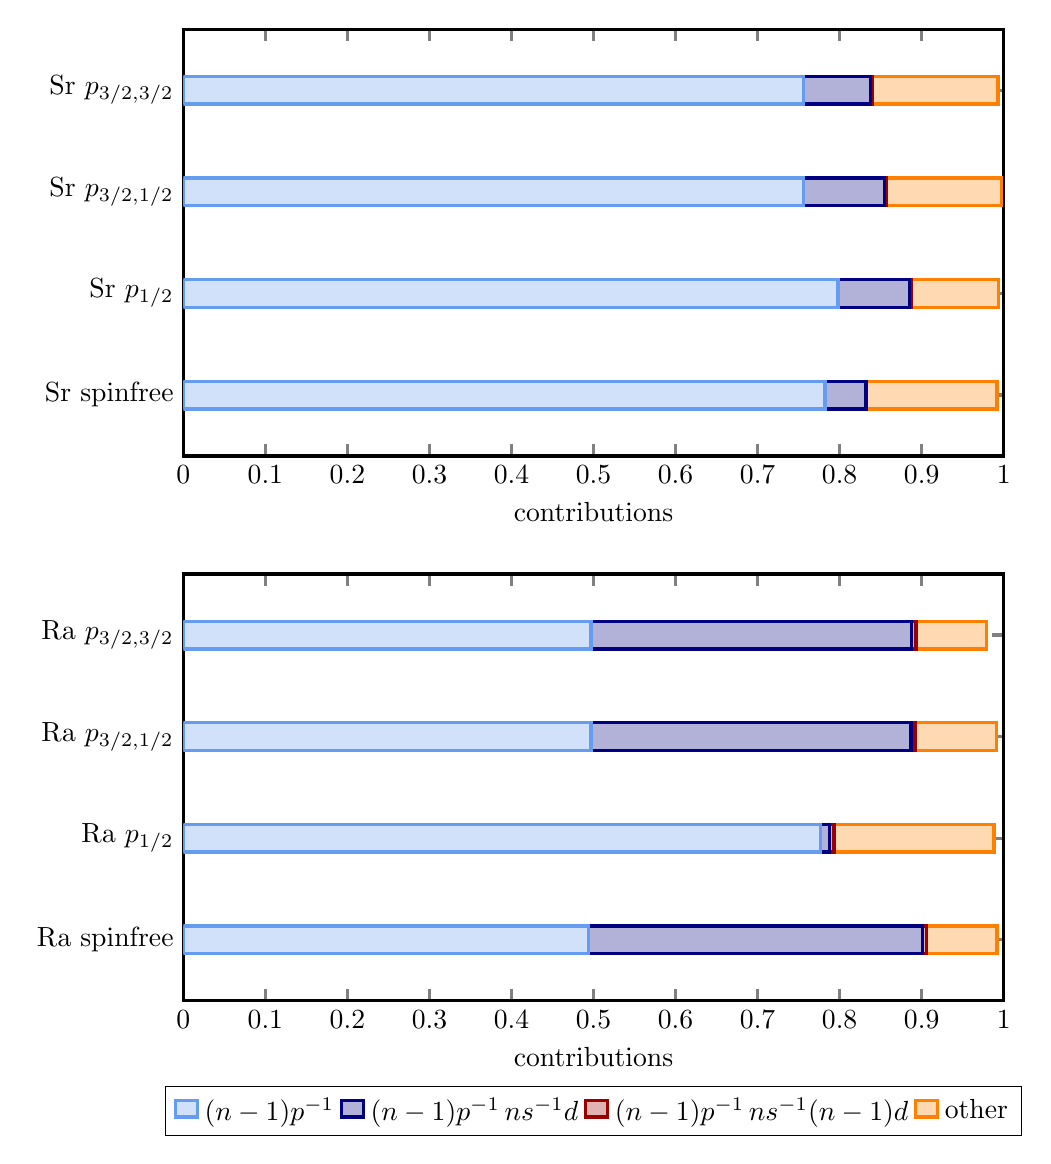
\begin{tikzpicture}
%\begin{axis}[
\begin{groupplot}[
     group style = {group size = 1 by 2, vertical sep=1.5cm},
     %enlargelimits=0.15,
     height = 7cm,
     width = 12cm,
     legend style={at={(0.5,-0.20)},
       anchor=north,legend columns=-1},
     xlabel={contributions},
     symbolic y coords={Sr spinfree,Sr $p_{1/2}$,Sr $p_{3/2,1/2}$,Sr $p_{3/2,3/2}$,
                        Ra spinfree,Ra $p_{1/2}$,Ra $p_{3/2,1/2}$,Ra $p_{3/2,3/2}$},
     %xtick=data,
     %nodes near coords,
     %nodes near coords align={horizontal},
     enlarge y limits=0.20, %space left and right
     axis line style = very thick,
     tick style = very thick,
     xbar stacked,
     xmin = 0,
     xmax = 1.0
    ]
    \nextgroupplot[xmin=0]
    \addplot+[xbar] coordinates {(0.782,Sr spinfree) (0.798,Sr $p_{1/2}$)
                          (0.756,Sr $p_{3/2,1/2}$) (0.756,Sr $p_{3/2,3/2}$) };
    \addplot+[xbar] coordinates {(0.050,Sr spinfree) (0.087,Sr $p_{1/2}$)
                          (0.099,Sr $p_{3/2,1/2}$) (0.082,Sr $p_{3/2,3/2}$) };
    \addplot+[xbar] coordinates {(0.000,Sr spinfree) (0.002,Sr $p_{1/2}$)
                          (0.002,Sr $p_{3/2,1/2}$) (0.002,Sr $p_{3/2,3/2}$) };
    \addplot+[xbar] coordinates {(0.160,Sr spinfree) (0.107,Sr $p_{1/2}$)
                          (0.140,Sr $p_{3/2,1/2}$) (0.153,Sr $p_{3/2,3/2}$) };

    \nextgroupplot[xmin=0]
    \addplot+[xbar] coordinates {(0.494,Ra spinfree) (0.777,Ra $p_{1/2}$)
                          (0.497,Ra $p_{3/2,1/2}$) (0.497,Ra $p_{3/2,3/2}$) };
    \addplot+[xbar] coordinates {(0.407,Ra spinfree) (0.011,Ra $p_{1/2}$)
                          (0.390,Ra $p_{3/2,1/2}$) (0.391,Ra $p_{3/2,3/2}$) };
    \addplot+[xbar] coordinates {(0.005,Ra spinfree) (0.005,Ra $p_{1/2}$)
                          (0.005,Ra $p_{3/2,1/2}$) (0.005,Ra $p_{3/2,3/2}$) };
    \addplot+[xbar] coordinates {(0.086,Ra spinfree) (0.195,Ra $p_{1/2}$)
                          (0.099,Ra $p_{3/2,1/2}$) (0.086,Ra $p_{3/2,3/2}$) };

\legend{$(n-1)p^{-1}$,$(n-1)p^{-1}\,ns^{-1}d$,$(n-1)p^{-1}\,ns^{-1}(n-1)d$,other};
  \end{groupplot}

%\end{axis}
\end{tikzpicture}




\end{document}
